\documentclass{article}

\usepackage{graphicx}
\usepackage{xspace}

\title{\emph{e[m]erge} work report 2}
\author{Stephen Sinclair, with Joseph Malloch, Sofian Audrey}
\date{May 30, 2012}

\newcommand{\emerge}{\emph{e[m]erge}\xspace}

\begin{document}
\maketitle

\section{Introduction}

This report describes developments in the \emerge project as of the
end of May, 2012.

\section{Data analysis}

In our context, the goal of data analysis is to determine useful ways
to look at sensor data such that it can be fed into a dynamic system
in order to generate responses.

An interpretation of ``useful'' here is that analysis should
well-characterise variations in the data such that interesting
features can be extracted.
In other words, we wish to perform dimensionality reduction, however
we also make use of standard supervised classification techniques in
order to evaluate the ability of reduced featuresets to predict data
tags.
If prediction is good, we can estimate that some combination of
features is ``useful'' for a dynamic system to respond to, and likely,
for driving media content.

Therefore we stress that classification is not the end goal of this
analysis, however it is a tool for examining the predictive quality of
features that we estimate from the raw data.
In this report we additionally use unsupervised methods for visual
inspection of separability in a severely reduced number of dimensions.

\subsection{Workshop 1 data}

The data from Workshop 1 was described and evaluated in the previous
report.
It consisted of subjects with accelerometers performing guided
gestures that might be typical of a concert environment.
The session was video taped and this was post-analysed to ``tag'' the
data with gesture information.

However, these tags were relatively unstructured and not every subject
was necessarily following the instructions at every frame.
Analysis was successful in separating low- and high-energy gestures.
More nuanced separation was not successful during analysis, possibly
due to a low sample rate of only approximately 10 Hz.

In the future we would like to revisit this data set using techniques
described in the following section, which may perhaps yield more
success, but as of the time of writing this has not yet been done.
On the other hand, if sample rate is indeed a problem as we suspect,
new data should be recorded.

\subsection{Lab data}

Six subjects were asked to perform five distinct gestures while
holding a Minibee wireless accelerometer.
A black dot was moved around on the screen, and the subjects were
asked to follow it with their hand, causing periodic or random motion
of various patterns.
The accelerometer was held in the fist.
This exercise provided us with pre-tagged data under a controlled
environment, which could subsequently be used as a basis for
evaluating data analysis methods.

\begin{figure}
a)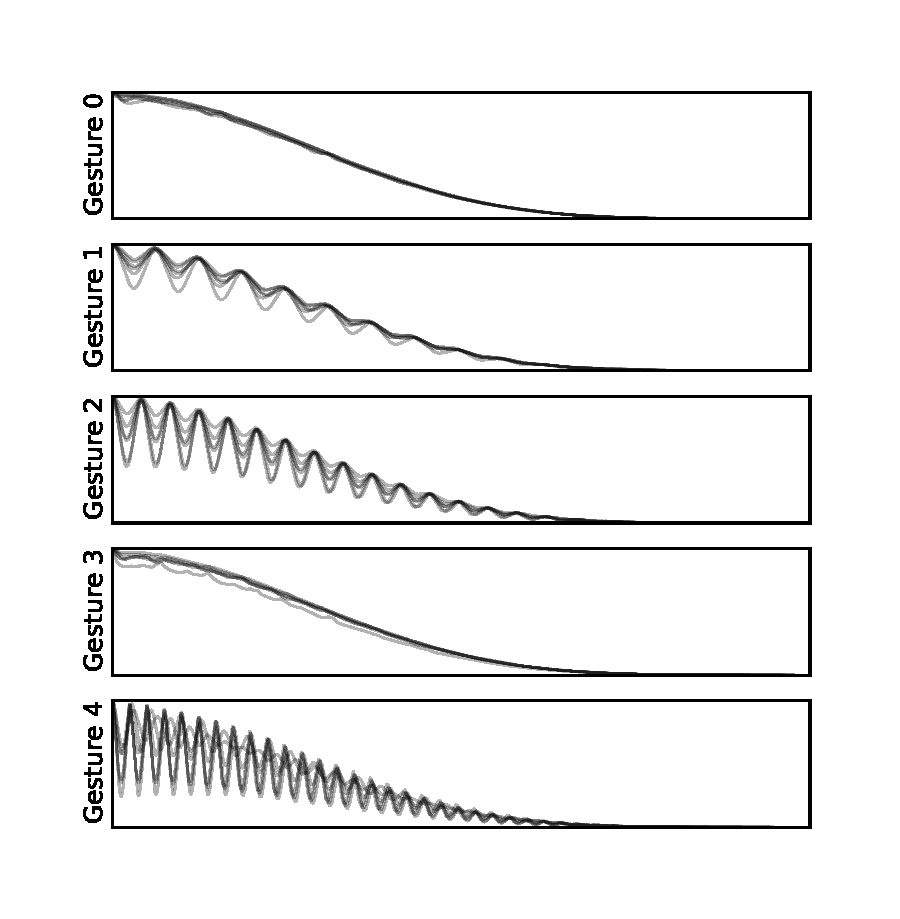
\includegraphics[width=2in]{autocor.pdf}
~b)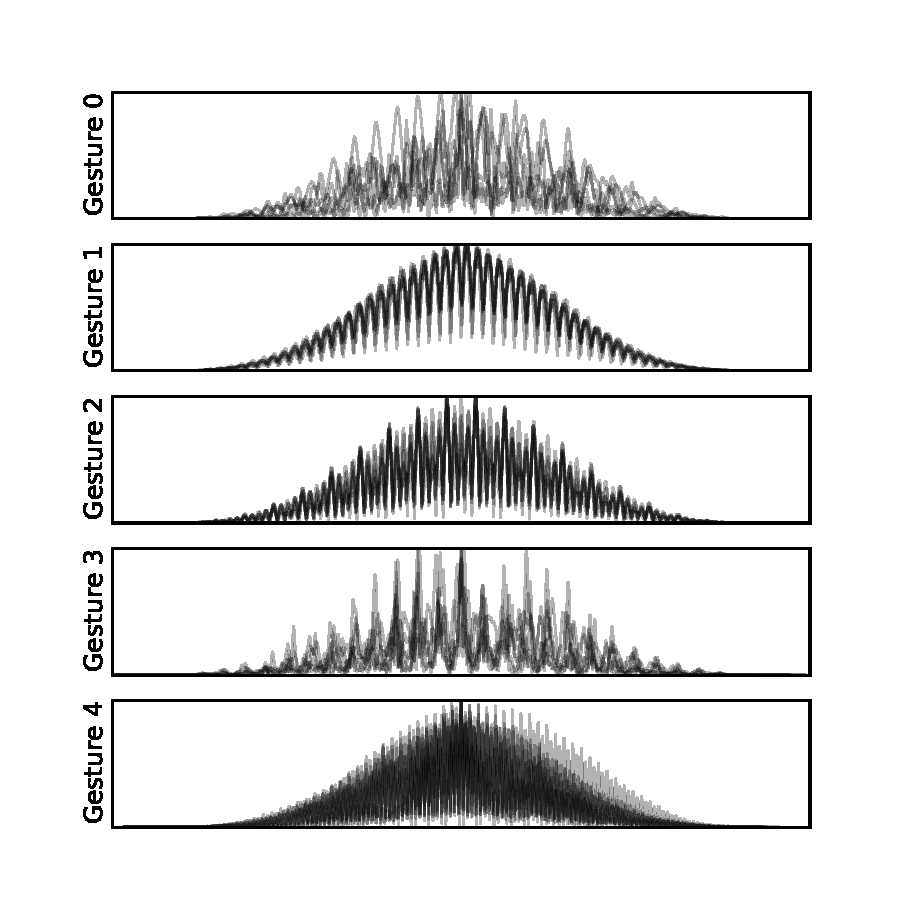
\includegraphics[width=2in]{axescor.pdf}
\caption{(a) Example magnitude autocorrelation vectors of lab data set
  separated by subject and gesture.
  (b) Example magnitude inter-axis correlation vectors of lab data set
  separated by subject and gesture.}
\label{fig:autocor}
\end{figure}

Initial investigation by comparing autocorrelation of the
accelerometer magnitude showed that gestures were mostly distinct, and
that there was some similarity between subjects.
Fig.~\ref{fig:autocor}a overlays one autocorrelation vector for each
subject and gesture, separated by gesture.

Use of magnitude autocorrelation as a feature for ANN prediction, seen
in Fig.~\ref{fig:autocor_ann}, resulted in classification that was not
completely satisfactory.
Although classification was successful for some gestures, several
gestures just barely classified.

\begin{figure}
\centerline{
  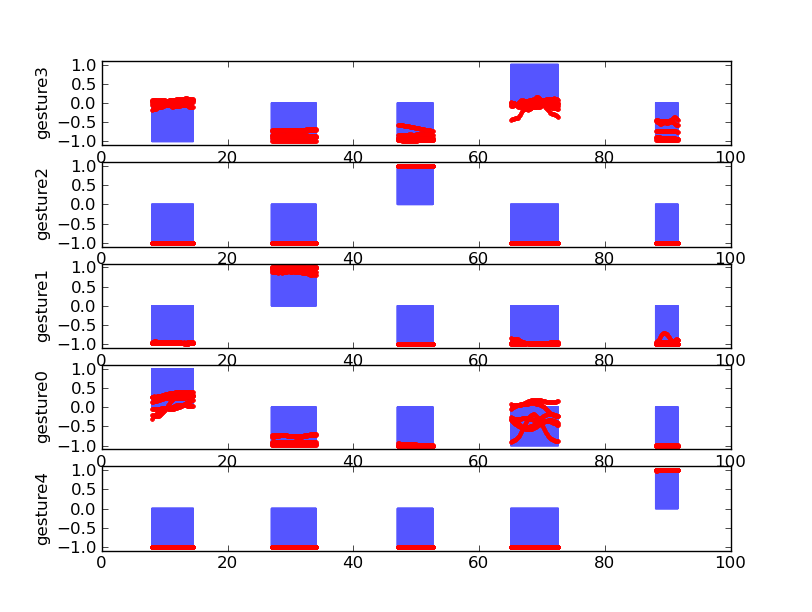
\includegraphics[width=4in]{autocor_ann.png}}
\caption{ANN classification results using magnitude autocorrelation.}
\label{fig:autocor_ann}
\end{figure}

However, taking the magnitude of accelerometer data necessitates
throwing out useful information about orientation.
On the other hand, calculating orientation explicitly has its own
problems: it requires removing of the gravity bias, and orientation
can be represented in several ways, requiring some choices.

\subsubsection{Inter-axis correlation analysis}

We decided that it would be more productive to attempt a more general
analysis method that takes into account rotation without explicitly
representing it.
The idea is to calculate the correlation between the three rotation
axes and take the sum of their absolute values.
This inter-axis correlation views the three accelerometer axes as
separate sensors and considers merely their mutual covariance.
A high-pass filter is used to remove gravity bias.

Other than this pre-filtering, this method is effectively agnostic to
specific information abou the sensor, therefore we hope it can be used
e.g.\ between sensors connected to kinematically-related bodies, or
even different types of sensors.
It is possible that summing the correlation vectors is also
unnecessary, and the whole set of three correlation vectors could be
used, however we found the sum to be an effective method of combining
the correlations.

Results are shown in Fig.~\ref{fig:autocor}b.
It can be seen that there is more variation between the gestures, yet
agreement across subjects is still quite good.
These results were also evaluated as classification features,
Fig.~\ref{fig:axescor_ann}.
It is clear that classification has been improved.

\begin{figure}
\centerline{
  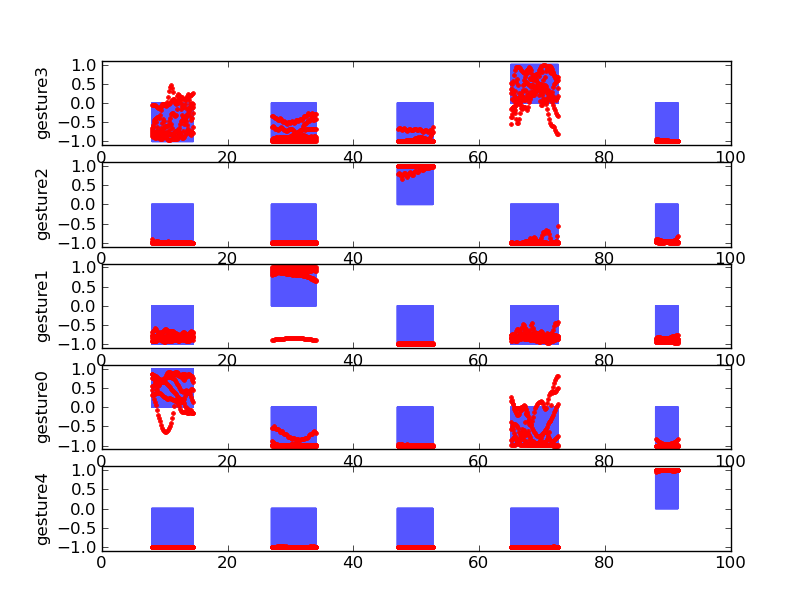
\includegraphics[width=4in]{axescor_ann.png}}
\caption{ANN classification results using inter-axis correlation.}
\label{fig:axescor_ann}
\end{figure}

\subsubsection{Data reduction}

Unfortunately these correlations provide very large feature vectors,
which would represent large amounts of data for exchange, and likely
impact real-time performance.
Currently we are using a 10-second buffer at 100 Hz, or 1024 points,
generating a correlation vector of 2048 points.
Per sensor, this could amount to a large amount of data to process.

We prefer to reduce the data to salient axes, giving two advantages:
1) Less data to transfer during real-time performance; 2) data
reduction can be performed on sending nodes, reducing the processing
requirement of the dynamic system host.

An initial attempt was based on the observation that the correlation
vectors tend to have a periodic structure.
This structure was ``summarized'' by calculating some standard
features used in periodic waveform analysis.
The fast Fourier transform (FFT) of the correlation vectors was
calculated, and the spectral centroid and slope were calculated
according to standard formulae.

\begin{figure}
\centerline{
  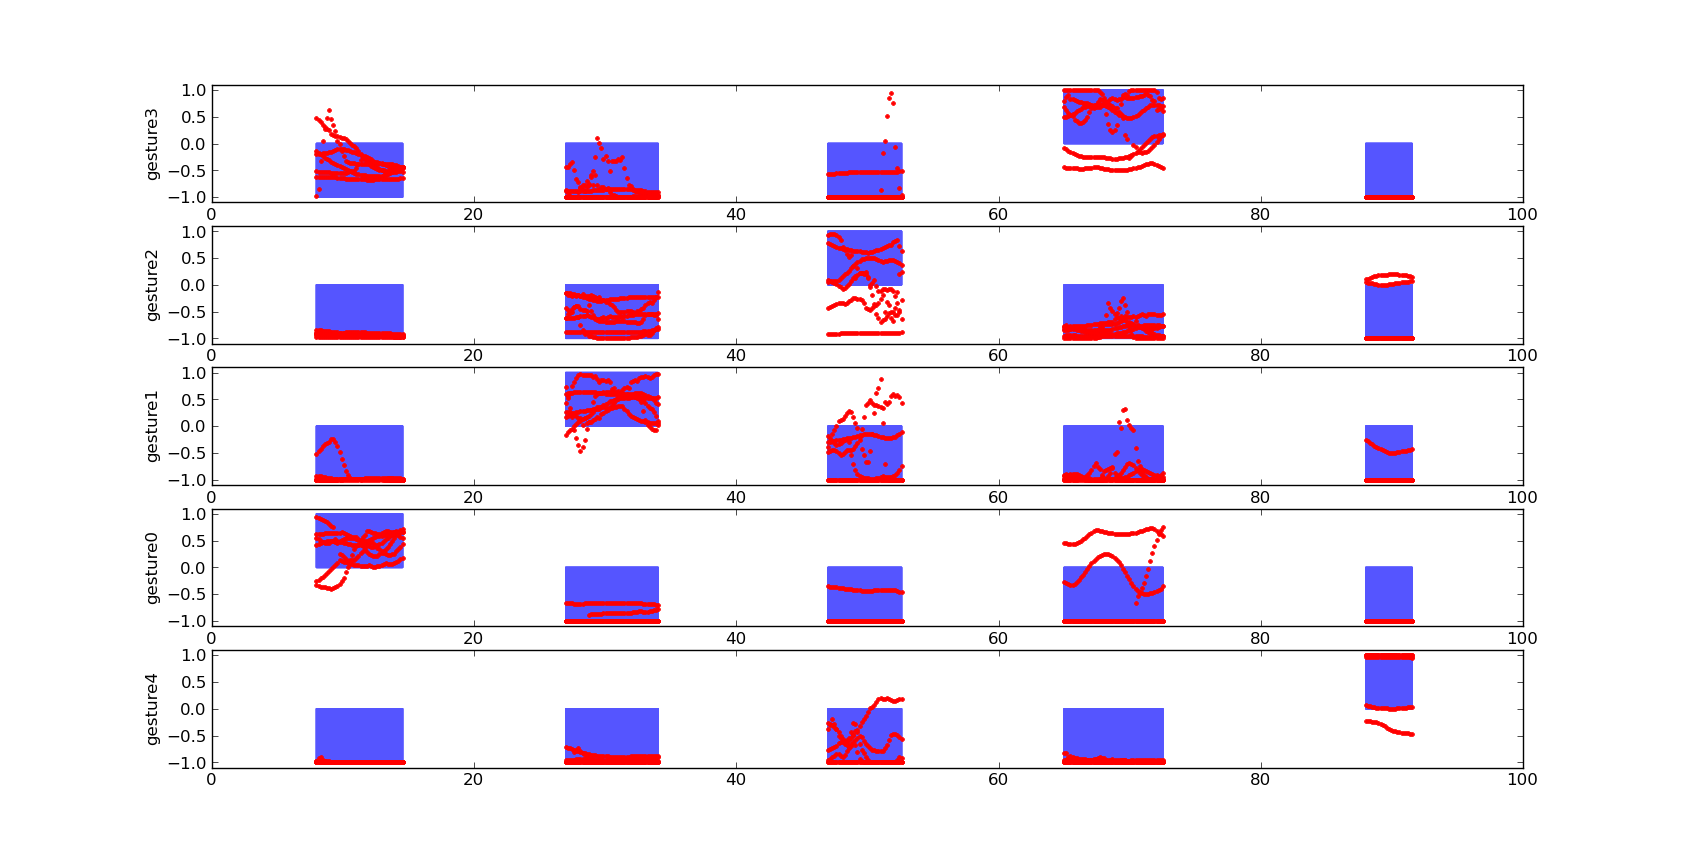
\includegraphics[width=4.5in]{reduced_ann.png}}
  \caption{ANN classification results using a reduced representation
    of the inter-axis correlation.}
\label{fig:reduced_ann}
\end{figure}

These two values were then used as features in classification, giving
results seen in Fig.~\ref{fig:reduced_ann}.
Although some misclassifications are obvious, the results are still
superior to those of the magnitude autocorrelation, with most data
being correctly classified.

\subsubsection{Instantaneous correlation}

Another method that was evaluated is the instantaneous correlation.
Since correlations may need to be performed locally on sensor nodes,
we sought a more efficient means of characterising sensor streams in
an online scenario.
In particular, the correlation methods described above require
processing a sliding window of 1024 samples.
Of course, different window sizes can be chosen, however the method of
instantaneous correlation described in \cite{Barbosa2012} replaces
this window with an exponential forgetting factor.
This allows efficient calculation of correlation using an IIR filter
representation.
Running several such filters at different delays allows the
construction of a 2D correlation matrix.

Examples of such matrixes generated from the lab data can be found in
Fig.~\ref{fig:instcor2d}.
These images were made with a 200 delays, and a filter cut-off
selected at 5~Hz.

\begin{figure}
\centerline{
  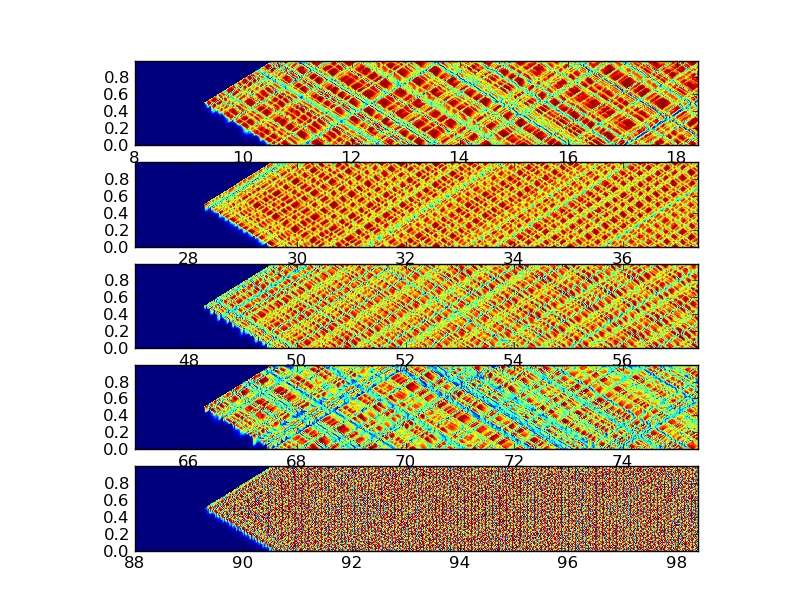
\includegraphics[width=4.5in]{instcor_5hz_200.png}}
  \caption{2-D instantaneous correlation of lab data at 5~Hz.}
\label{fig:instcor2d}
\end{figure}

It can be seen that each gesture generates a distinct pattern.
Therefore this method shows promise in identifying gestures.
Unfortunately, since the forgetting factor emphasises recent data
above old data, it leads to a ``sliding'' behaviour in the
characteristic pattern over time.
This makes the use of this data for recognition at any particular time
slice difficult.
Moreover, at mistuned cut-off frequencies, we found that this pattern
was much less distinct, therefore tuning is an important consideration
for using this method.

We tried using such vectors as classification features but this did
not perform well, presumably due to the time-varying nature.
We also tried using the FFT of the instantaneous correlation vector
and comparing only the magnitude, so as to ignore phase information,
but this did not yield greater success.

Therefore, we conclude that more research is needed to make use of
instantaneous correlation, however there are indications that it could
be worth pursuing since it lends itself well to real-time constraints
and smaller memory loads.

\subsubsection{Principal component analysis}\label{sec:pca}

\begin{figure}
\vspace{-1in}
\centerline{
  a)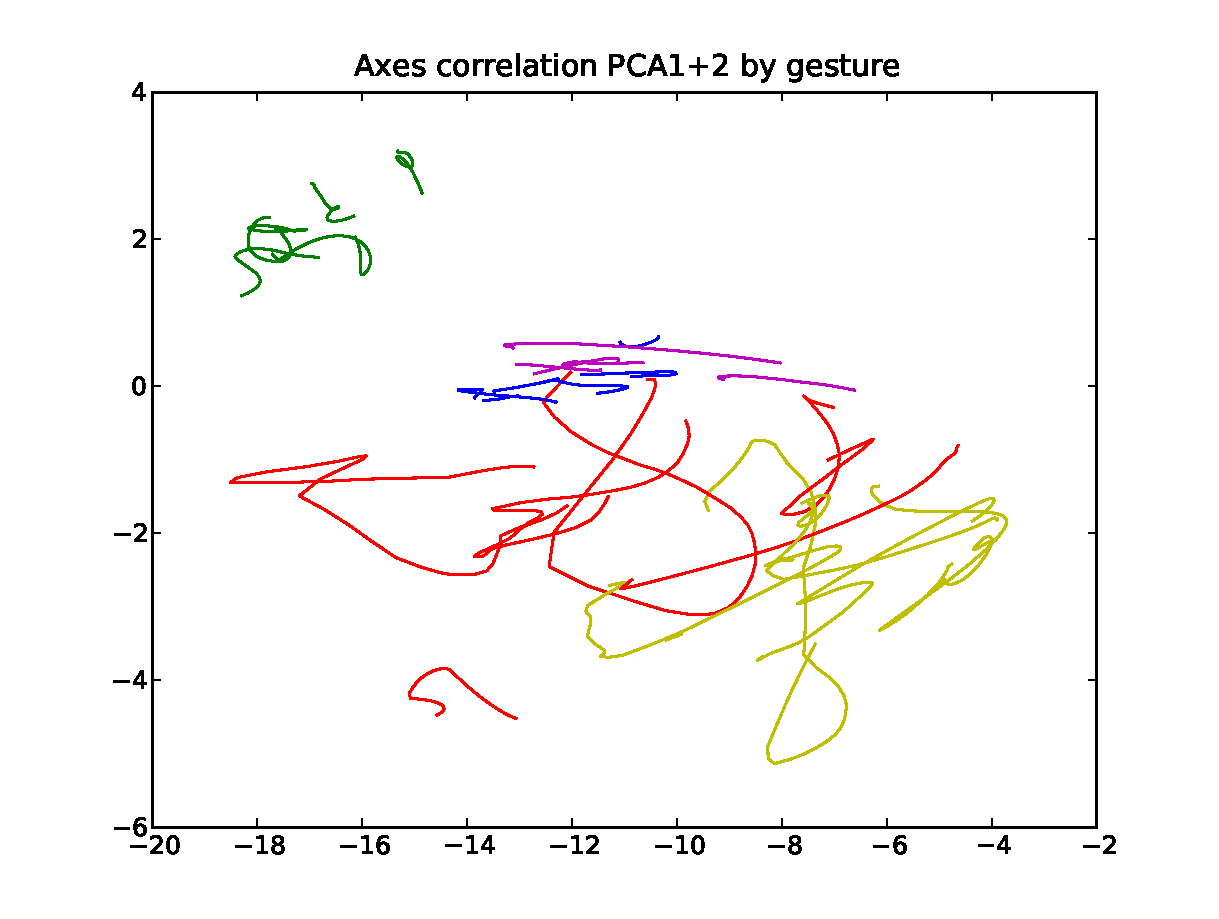
\includegraphics[width=3.5in]{pca_axes_cor_by_gesture.pdf}
  b)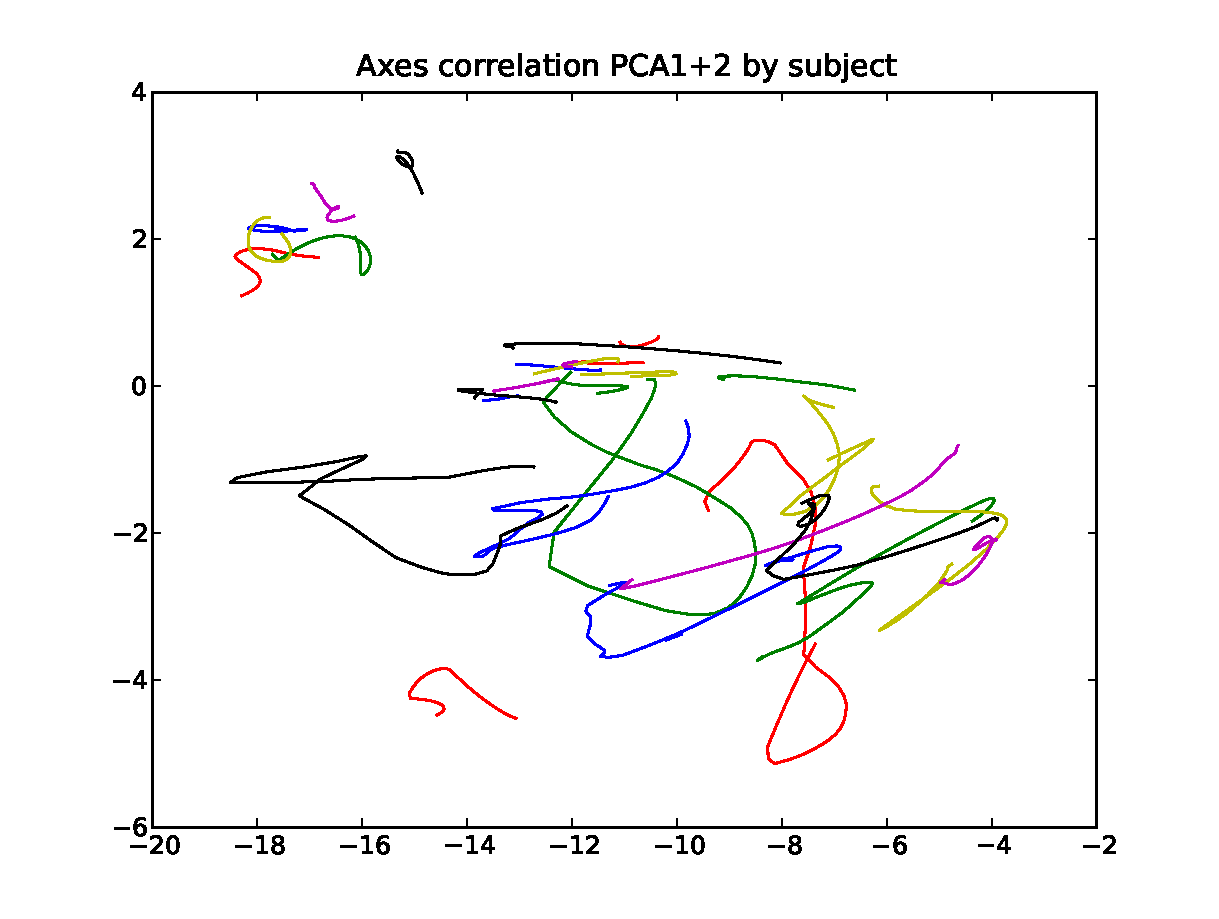
\includegraphics[width=3.5in]{pca_axes_cor_by_subject.pdf}}
\centerline{
  c)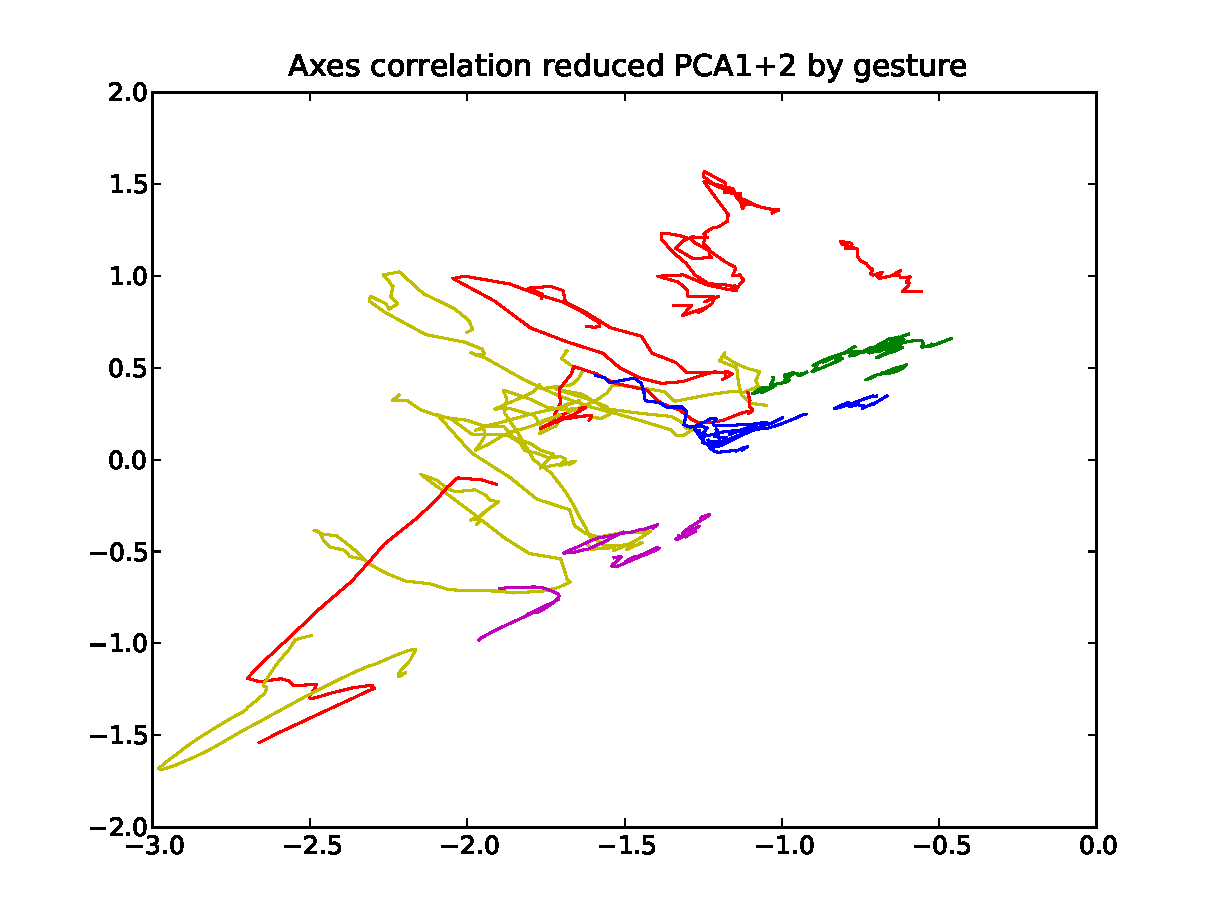
\includegraphics[width=3.5in]{pca_axes_cor_reduced_by_gesture.pdf}
  d)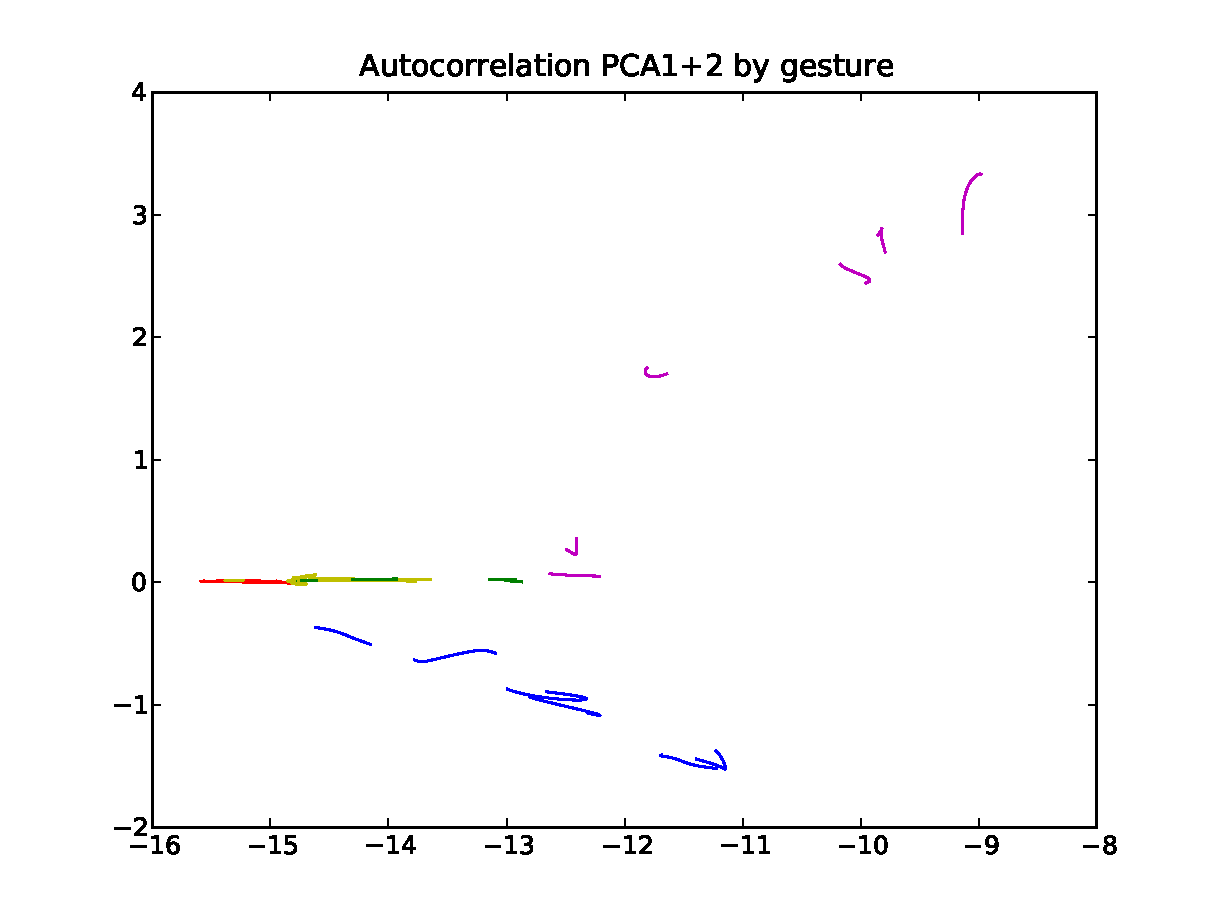
\includegraphics[width=3.5in]{pca_autocor_by_gesture.pdf}}
\centerline{
  e)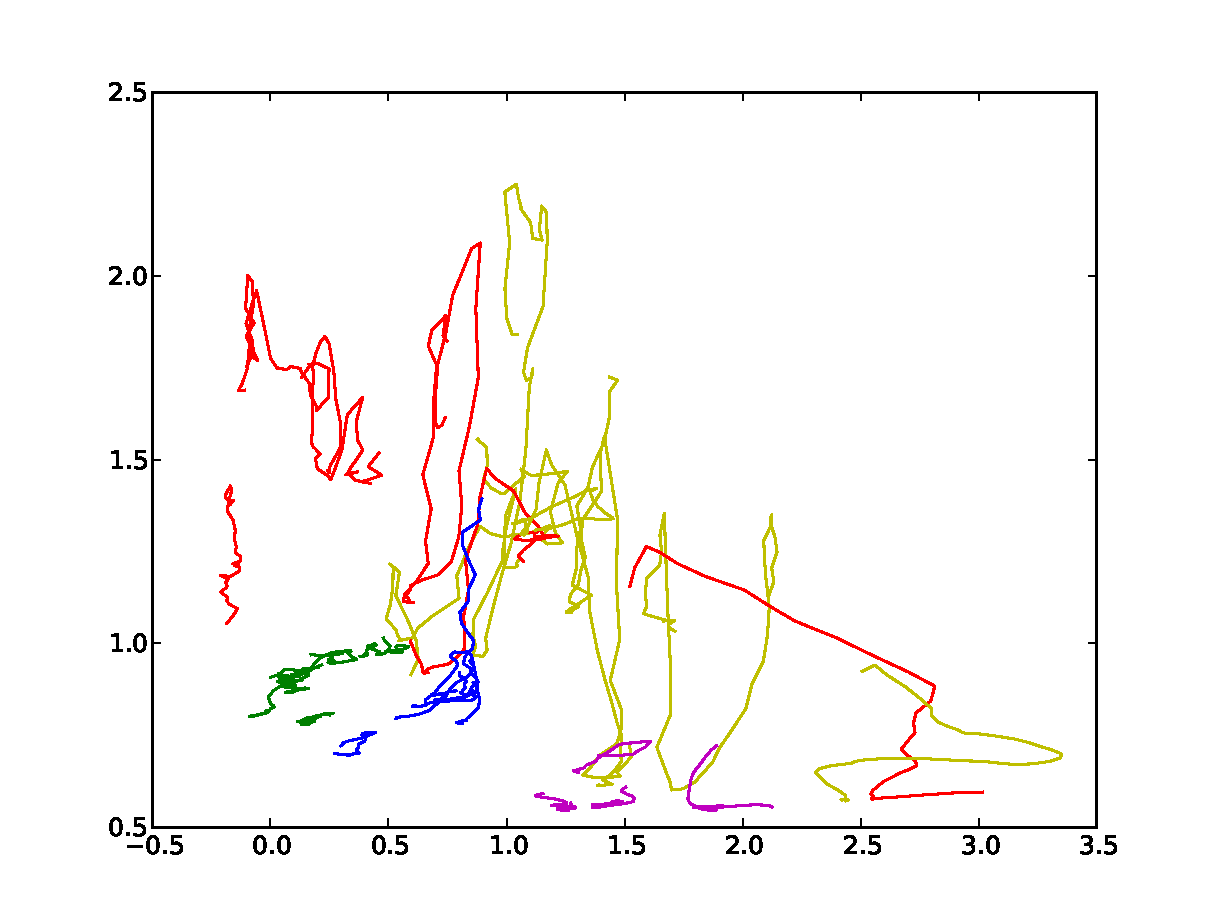
\includegraphics[width=3.5in]{reduced_cor_by_gesture_lines.pdf}}
  \caption{Two first principal components of: (a) Inter-axis
    correlation coloured by gesture, (b) coloured by subject, (c)
    Reduced representation of inter-axis correlation coloured by
    gesture, (d) Autocorrelation coloured by gesture. (e) Reduced
    inter-axis correlation measures without PCA.}
\label{fig:pca}
\end{figure}

Principal component analysis (PCA) can be used to identify ``why'' and
``whether'' certain feature sets may provide good separation.
This can be viewed as an alternative method to using classification to
evaluate feature sets.
It is considered an unsupervised learning method in the sense that the
data is used to determine a transformation to a more useful
representation, without reference to external information such as
tags.

Some unsupervised techniques such as $k$-means analysis perform
clustering, however PCA merely determines a change in coordinates such
that a new ``view'' on the data maximally spreads out the variance in
the new coordinate system.
In the sense that it should reduce data to a minimal number of salient
dimensions, it can be considered an optimal way to view data in a
reduced number of dimensions.
Thus, by plotting the first two principal components, we may see how
much variance is in the data on a 2-D graph.

This result is given in Fig.~\ref{fig:pca}.
In Fig.~\ref{fig:pca}a, the two first PCs of each gesture is plotted,
coloured by gesture, and we can see that each gesture tends towards
its own part of the space.
Thus we can say that this data is separable.
On the other hand, in Fig.~\ref{fig:pca}b, the same lines are coloured
by subject, and it is noticed that subjects are not separable according
to their gestures.
This suggests that subjects had a good degree of consistency between
them, and very little consistency between gestures.

Similarly, the 2 PCs are also plotted for the reduced representation,
in fig.~\ref{fig:pca}c.
The separability between gestures is not as high, but still present.
In comparison, the 2 PCs are plotted for the magnitude autocorrelation
in fig.~\ref{fig:pca}d, and it can be seen that some gestures are much
closer together, while several strokes of the same gesture are further
apart.

Since our reduced inter-axis correlation representation is
2-dimensional, i.e.\ the spectral centroid and slope, we can also show
this plot for comparison with PCA.
In fig.~\ref{fig:pca}e, it is clear that PCA transformation is not
needed for this representation, since it is already nicely separable
by gesture.
Indeed, the PCA essentially just provides a simple rotation of this
space.

Overall, the results of PCA seem to indicate a good agreement with our
ANN-based classification analysis presented above.
However, PCA lends itself nicely to lower-dimensional representation,
which will come in handy during the discussion of visualization,
below.

As mentioned, however, it is still to verify that these techniques
apply well to general, unstructured accelerometer data as we might
receive from sensors in smartphones for example.
Larger data sets may be needed, and in that case comparison with
reliable tags may be impossible, therefore unsupervised methods may be
preferred.
Unfortunately, without tags, it will nonetheless be difficult to infer
\emph{meaning} in the results of unsupervised methods.
But a large data set may help to establish points of interest and
general boundaries of a PCA space that we may wish our system to react
to.

\section{Dynamic systems}

In addition to data analysis, an important component of the \emerge
project is the use of dynamic systems to react to sensor data and
provide feedback by means of media control.
We have developed two systems which can work together or independently
to provide a dynamic response to sensor input.

The first is a library for agent-based behaviour, written by Sofian,
called Qualia.
The other is a shared environment called Influence, written by Joe and
Steve, which uses a pixel-based, GPU-driven 2-D convolution process to
iteratively transmit information between agents that inhabit the
space.
Using libmapper as a communication protocol, Qualia can control agents
which inhabit the Influence environment, but Influence can also be
inhabited by agents reacting in a purely physical manner (particles),
or by agents controlled externally by human input.

\subsection{Qualia}

Qualia is a C++ library which provides a framework for development of
agent-based logic.
In particular, it implements subsystems for reinforcement learning and
for state machines.

Reinforcement learning is an interesting approach because the designer
need not understand the mechanics of the agent's decision making
process.
Rather, the designer can focus on what the intended behaviour is by
creating a ``reward function,'' which rewards the agent for good
behaviour and punishes it for bad behaviour.
Over time, the agent will learn to associate its own actions and its
observations of its environment with good or bad behaviour, and try to
perform ``good'' actions.

In order to test the idea as an interactive system, we decided to
implement a simple one-on-one interaction between a Qualia agent and a
human.
An applet was developed in Processing which accepted human input via
mouse motion and button state.
A circle was made to follow the human by applying spring forces
towards the mouse position, and the mouse button state controlled the
polarity of a virtual magnet attached to this circle.

The agent also controlled a circle, and its action could only turn the
magnet on and off.
Therefore if the polarities of the human and agent were the same, the
agent would be attracted towards the human, or otherwise repelled.
The reward function was designed to reward the agent for getting close
to the human within a certain radius, however, if this radius was
surpassed and the agent got too close, it would be punished heavily.
Therefore the agent tried to learn how to approach the human without
getting too close.
Later, we allowed the human to control the system using a Minibee,
pictured in Fig.~\ref{fig:qualia_minibee}.

\begin{figure}
\centerline{
  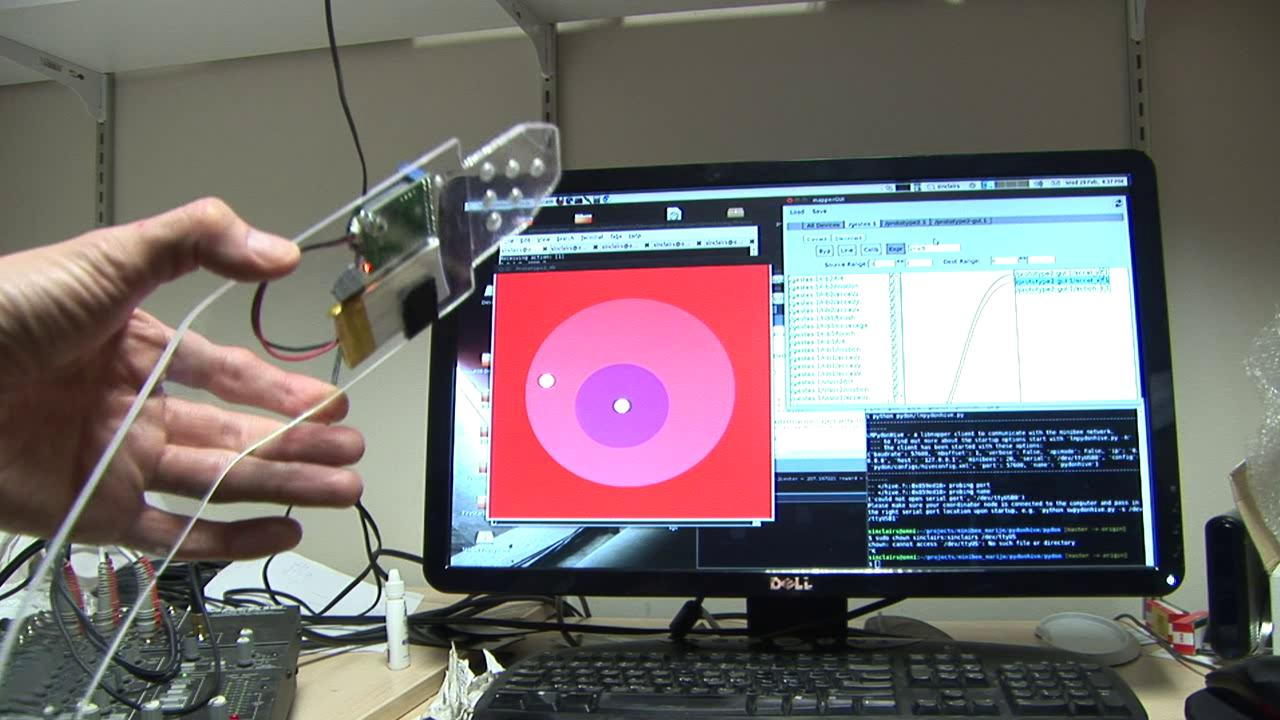
\includegraphics[width=4.5in]{qualia_minibee.jpg}}
  \caption{Qualia interacting with a human.}
\label{fig:qualia_minibee}
\end{figure}

The impression was interesting.
Although the agent is clearly trying to get close, it feels very
tentative at first.
However, this encourages the human to try to ``taunt'' the agent and
bring it out into the center.
We also found that it sometimes ended up in corners, therefore we
added rules to punish it for being too close to the sides.

After some time, we found that we started to play with the agent,
trying to attract it and see how close we could get.
In other words, we started playing a collaborative game with the
agent.
The magnetic physics caused the agent to fly away quite quickly when
it came too close, due to the distance-squared forces, which added to
the fun.

This system also demonstrated the use of libmapper as a transport
layer between an agent, an environment, and a human.
Qualia, the Processing applet, and the Minibee ran in different
processes, usually on different computers in the IDMIL.

Next, we planned to determine how to scale this interactive design in
order to involve multiple users and multiple agents.
This led to the development of the Influence environment, detailed in
the next section.

\subsection{The Influence environment}

An immediate idea for involving multiple agents was to have them
connect to the Processing environment just like the original Qualia
agent, and have the Processing physics engine apply forces between
them.
However, with a mind towards generalization and scalability, we wanted
to make such an environment where the motion of agents was determined
mostly by the agents rather than the central process, so that no one
process was in charge of integrating all the physics.
In the setup above, the physics engine inside the Processing applet
would be in charge of an N-body physical problem, which may not scale
well to large numbers of agents.

Additionally, although the physical motion was an interesting
interaction, we wanted an environment which could be used in a more
general way, to inform agents of their surroundings and allow them to
make decisions on how to act, without needing to implement globals
laws such as a physical simulation.
The reason is that the locations of agents in this space will not
necessarily represent physical positions, but may indeed be used to
represent characteristic analyses of sensor data.

Previously in the IDMIL, Joe had designed an interactive table which
used a pixel-based convolution method to transmit information about
what objects are on the table towards objects in a physical
simulation.
At each iteration, 30 frames per second, the convolution caused active
pixels to spread further and further, and meanwhile a physics engine
was reading the pixel data and using it to inform forces; this allowed
simulated objects to be attracted or repelled by real objects seen
through a camera.

We decided to use this idea to propagate information between agents.
This has several advantages for our application: firstly, the N-body
problem enabling all agents to ``see'' all other agents is spread
across time, so that it becomes a linear problem in the number of
pixels rather than agents.
Although this could be represent considerable amount of processing, we
implemented the convolution in a GPU shader, off-loading the work from
the CPU.
Since it does not increase with the number of agents, as long as the
GPU can handle the workload, computational requirements are constant.
Secondly, since interaction takes place in a 2-D bitmap, it lends
itself to other methods of interaction, such as drawing directly on
the surface, placing virtual walls or objects in the space, or taking
input from a video or depth camera such as the Microsoft Kinect.

\begin{figure}
\centerline{
  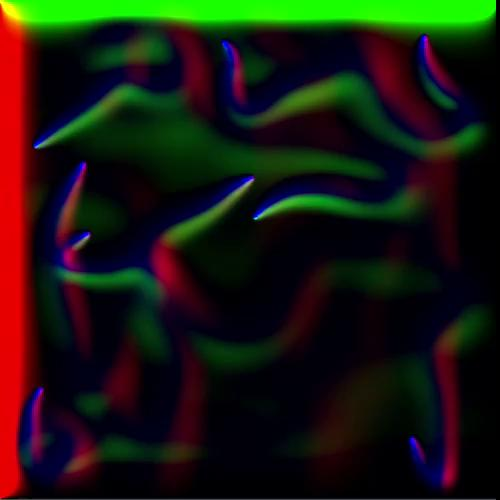
\includegraphics[width=2.5in]{influence.jpg}}
  \caption{The Influence environment with several physical agents
    connected.}
\label{fig:influence}
\end{figure}

The current implementation features 2-D vector fields that support
directionality, enabling effects such as spin and flow.
The user can draw flows with the mouse that pull agents along a path.
Currently we have connected physical agents that simply react to
observations, the values in surrounding pixels, with force in some
direction.
It can be seen in Fig.~\ref{fig:influence} that the agents leave
trails.
This is because as they move, they write values to the vector field
which decay over time.

At the Moment Factory work session in May, we have also connected a
Qualia agent and used MF's X-Agora software to display agent positions
by mapping to it using the libmapper GUI.
The Qualia agent did not behave in an interesting way, so the reward
function needs work, however as a proof of concept the trial was
successful.

There are some limitations.
Since they also write in front of themselves, they tend to see their
own influence, which limits the speed at which they can move.
Additionally, an agent in motion can only affect agents that happen to
move behind it.
It is possible to use additional passes or larger convolution kernels
to increase the speed of influence propagation, however this has
strange effects on their motion, again due to them seeing their own
influence.

Nonetheless, Joe has implemented some test environments with large
numbers of local agents, which can be seen in
Fig.~\ref{fig:manyagents}.
These show that interesting emergent behaviour can arise by having one
or two types of agents with simple sets of rules.

\begin{figure}
\centerline{
  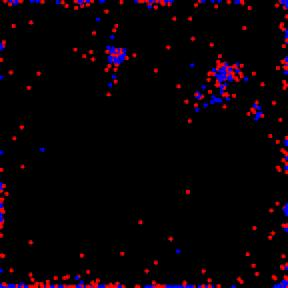
\includegraphics[width=1.3in]{quasi-stable_molecules.jpg}
  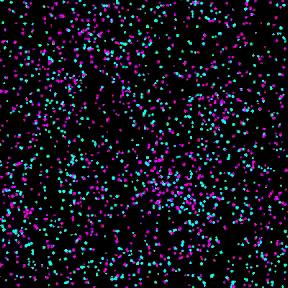
\includegraphics[width=1.3in]{emergent_opposing_flows.jpg}
  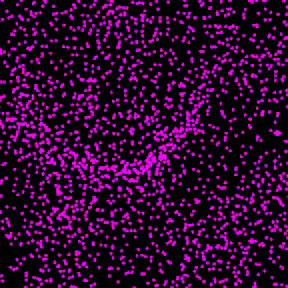
\includegraphics[width=1.3in]{emerging_flows_one.jpg}
  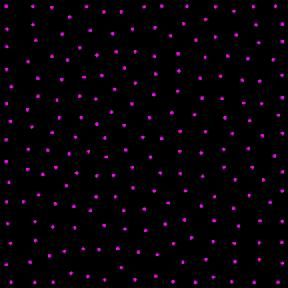
\includegraphics[width=1.3in]{stable_repulsion.jpg}
  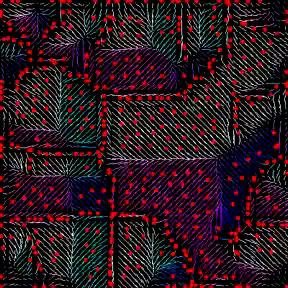
\includegraphics[width=1.3in]{membranes.jpg}}
  \caption{Large numbers of physical agents in the Influence
    environment creating various emergent effects. Left to right:
    quasi-stable molecules form; opposing flows; flows give rise to
    waves; stable repulsion; spacial division into membranes filled
    with repulsive particles.}
\label{fig:manyagents}
\end{figure}


Even if the cited limitations pose a problem, Influence presents a
proof of concept dynamic environment where agents of different types
can inhabit and observe each other.
A physical environment such as a gravity simulation could provide
similar communication.
Either way agents will need a way to summarize information about
surrounding agents such that their information can be reduced to a
constant-sized vector which can be processed by some decision engine
such as Qualia's reinforcement learning.

We have shown that a dynamic system can be fed information from
sensors, simulations, and intelligent agents, such that they observe
each others behaviour and react.

A possible use case for this software will be to use agent positions
to represent data other than physical position.
For example, the PCA transform used to analyse the gesture data in
section~\ref{sec:pca} may be applied to incoming sensor data and used
to position agents within the Influence environment.
Since their position now represents the gestural activity, after a
short moment agents will be able to tell that there are other agents
behaving in a similar manner.

A reinforcement agent could notice that its actions cause activity in
a certain region, and respond with some media to encourage more human
agents towards a given location, or attempt to disperse them from some
activity that is getting boring.

\subsubsection{Scalability}

Currently Influence can be connected with tens of agents, it has been
run with about 100 agents connected at once.
In the future we would like to connect many more agents.
This is mostly a communication bottleneck; if some agents such as
physical agents or Qualia agents are run locally to the process, many
more can be supported, as Joe has shown by running thousands of
physical agents in real time.

Therefore if network communication is reserved for sensor-based agents
and off-loaded computation only if necessary, we estimate being able
to increase the total number of agents in the system.
Eventually we expect that the number of sensors connected to a single
computer will be the main restriction.
At that point, ideas for expanding the environment idea to a
decentralized approach will be necessary; these include stitching
together several Influence environments running on separate computers
by transmitting border pixels, or having other methods of multiple
Influence environments to perturb each other.
(E.g.\ agents which jump from one environment to another depending on
some state.)

In any case, if this kind of interactivity is to scale to thousands or
tens of thousands of cell phones for example, more serious
consideration to hardware and software designed for this purpose will
be required.

\section{Visualization and media}

Thus far not much thought has gone towards visualization and media
throughout the \emerge project, however consideration of interacting
with content is a necessary project goal.

One very simple idea has been to take the natural colour mapping used
in Influence and use this to map images to a video feed.
An example is given in Fig.~\ref{fig:influenceblend}, where images of
the four seasons were downloaded from Flickr and blended according to
rules governed by the pixel colours.

\begin{figure}
\centerline{
  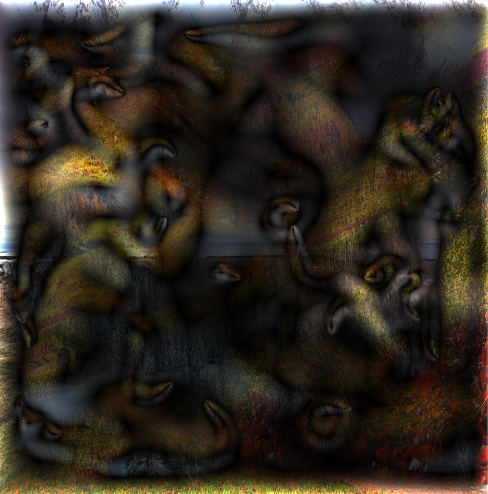
\includegraphics[width=3in]{influence_blend.png}}
  \caption{The Influence environment with images of 4 seasons mapped
    to the colour space used to maintain the vector fields.}
\label{fig:influenceblend}
\end{figure}

Another idea has been to project the agents on the floor, and use a
Kinect feed to have physical or intelligent agents swarm around
detected humans and objects.

However, more seriously we presume that the positions of agents and
their influence will not be directly mapped to media, but will be used
to observe activity in certain regions of the gesture space.
This will indirectly control some media through decision logic, either
intelligent or explicitly designed, to encourage or discourage such
activiy, as suggested above.
They may consist of dimming or brightening lights, controlling video
projections, or anything else.
This part of the project is still under discussion, however progress
has been made in connect other \emerge projects to X-Agora via
libmapper.

\section{Libmapper progress}

Throughout the work described in previous sections, libmapper, liblo,
and surrounding software have seen a great amount of attention toward
supporting current and future \emerge development.

Libmapper has been completely ported to Windows, currently compiling
using the MingW/MSYS Unix-like environment for Windows.
Visual Studio support for libmapper is in the works, since it has been
requested by Moment Factory.
It has not been immediate since it means removing some C99'isms in the
code base which are not supported by the Microsoft C compiler.

Tentatively, Android support has also been in the works.
Mostly liblo has been made to compile in the Android NDK, however
testing of libmapper is still down the line.
Moment Factory's current interest in cell phones is over the HTML5
mobile API, therefore getting native support into Android and iOS has
not been a major priority.

Additionally, as mentioned above, Moment Factory's contribution has
been to incorporate libmapper into their X-Agora software via the
built-in Lua interpreter, work done by Bruno Angeles, which allows
remote programs such as Influence to control elements in its
scenegraph for visualization purposes.
In the MF work session in May, we also used their HTML5 back-end with
libmapper through the Max/MSP object, which has been ported to Windows
for this purpose.

The major undertaking for libmapper itself in the last few months has
been Joe's work on the ``instances'' feature, which will lend itself
well to the Influence environment in order to support an arbitrary
number of agents.
This feature is also necessary for other libmapper purposes, such as
to support multitouch mapping and polyphony in musical contexts.

Instances have been working for some time, but not yet integrated into
the main development branch due to continuing thought toward design
decisions, as well as difficulty finding time for the team to fully
review code changes, which are non-trivial.
Recently, experience with bidirectional communication between agents
and Influence have also led to some surprisingly tricky issues in the
connection logic which are currently being ironed out.
For details we refer the reader to the libmapper mailing list where
discussion is on-going.

Currently we are successfully testing ideas in Influence without
instances, but when instances are made available in the main code
branch it will ease testing, experimental mapping, and scalability
when dealing with large numbers of remote agents.

\section{Vibrotactile feedback}

As a somewhat peripheral project, Marcello Giordano (IDMIL) has
investigated control of the Android vibration API.
He has designed an application which can respond to user interaction
or incoming OSC messages to stimulate vibration signals to the user.

This could be used in the future as a response mechanism in synchrony
with media, or could be used directly for cell phone interaction to
encourage usage of gaming interfaces for interactive control of an
agent.

\section{Conclusion}

To date we have managed to find methods for reducing dimensionality of
correlations based on accelerometer data, and incorporated these
results into real-time controls for agents in a dynamic system.
Examining the working \emerge system diagram, Fig.~\ref{fig:system},
we can see that most of the boxes have been covered thus far.

Data Collection has been addressed by the Minibees and continued work
on cell phone integration at MF.
Feature extraction has been examined in a lab context and successfully
used to determine salient features, though it continues to be a point
of research in regards to more natural data.

Off-line visualization and classification have been used to examine
salience of data analysis methods.
In the ``field,'' it may be interesting to develop real-time PCA tools
or other unsupervised methods for active visualization of crowd
behaviour.

We have developed dynamic systems and intelligent agents able to react
and interact with sensor data.
Although all these directions will continue to require research and
development, it is clear that the main focus left for this project is
to integrate the above systems into active media control.

This is planned as a major upcoming subject for the next \emerge
meeting and an active topic through the summer to wrap up the project.

\begin{figure}
\centerline{
  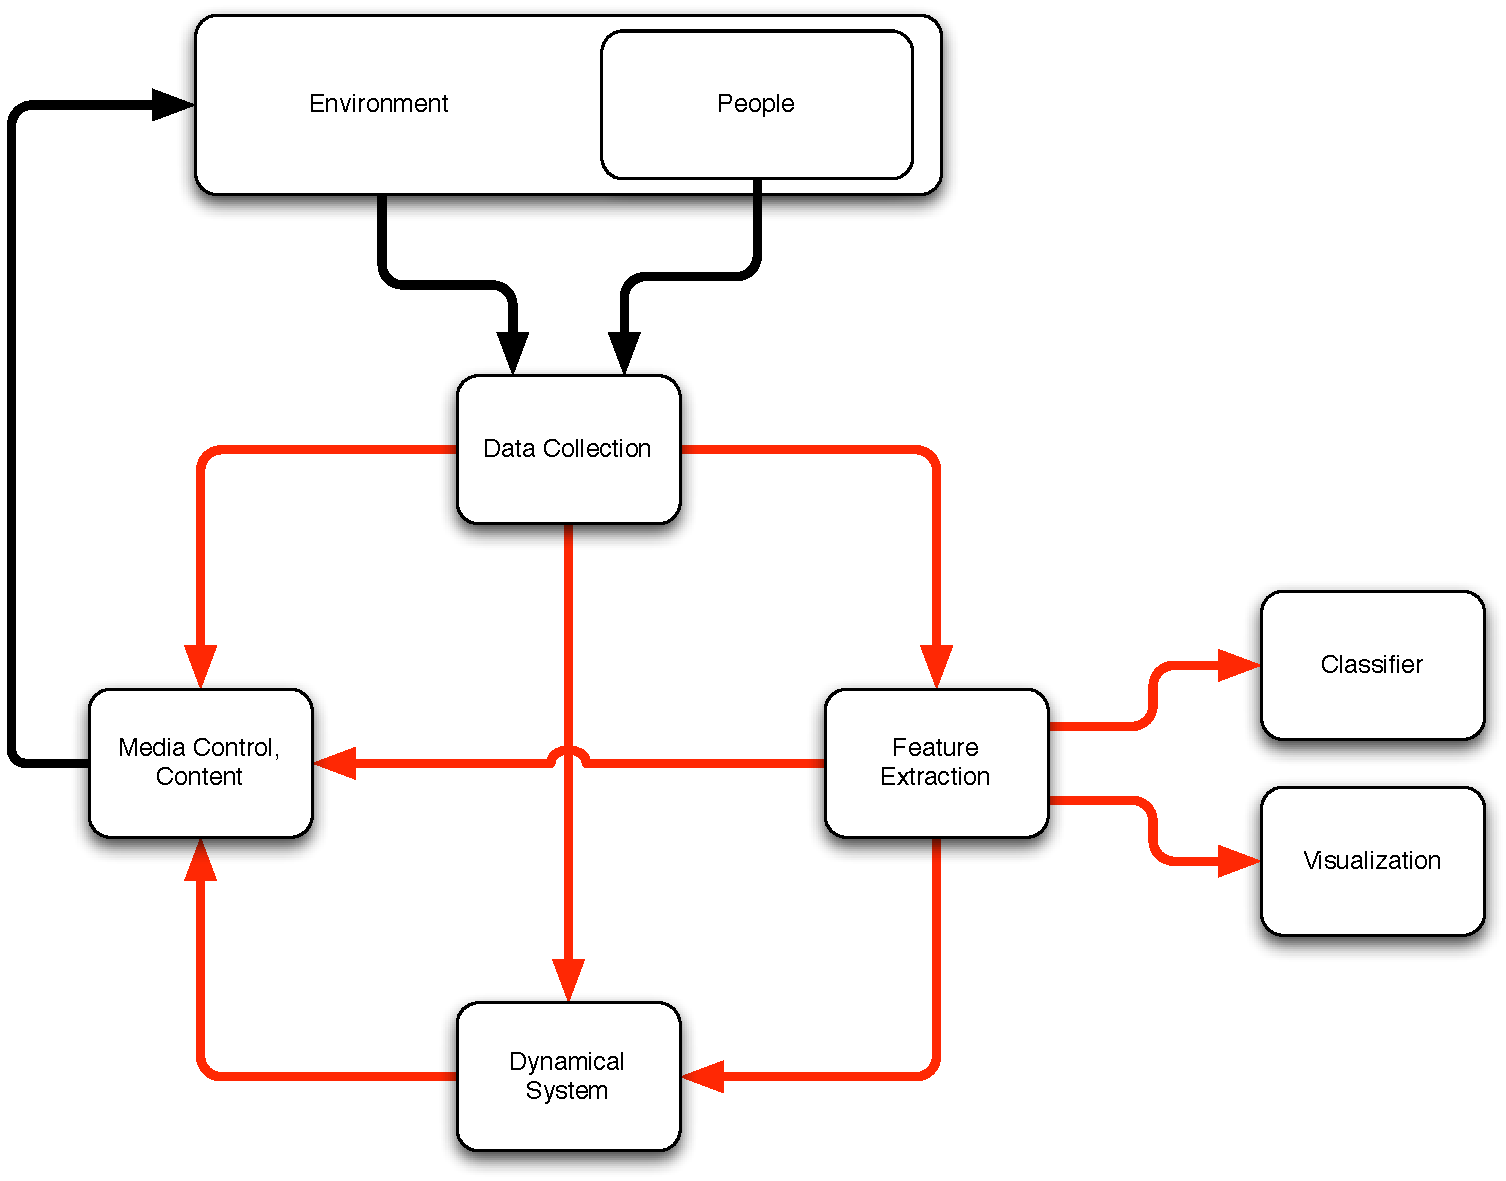
\includegraphics[width=4.5in]{system_diagram.pdf}}
  \caption{System diagram for \emerge.}
\label{fig:system}
\end{figure}

\bibliographystyle{abbrv}
\bibliography{references}

\end{document}
